\chapter{LLM Agentic Training}
\label{llm-agentic-training}

\section{Motivation: From Chatbots to Autonomous Agents}
\label{motivation-from-chatbots-to-autonomous-agents}

Modern LLMs are increasingly deployed not just as conversational assistants but as \textbf{autonomous agents} that interact with external tools, APIs, databases, and environments over multiple steps. This shift---from single-turn chatbots to multi-step agents---introduces fundamentally new RL challenges that require rethinking how we train, evaluate, and deploy language models.

\begin{figure}[ht!]
\centering
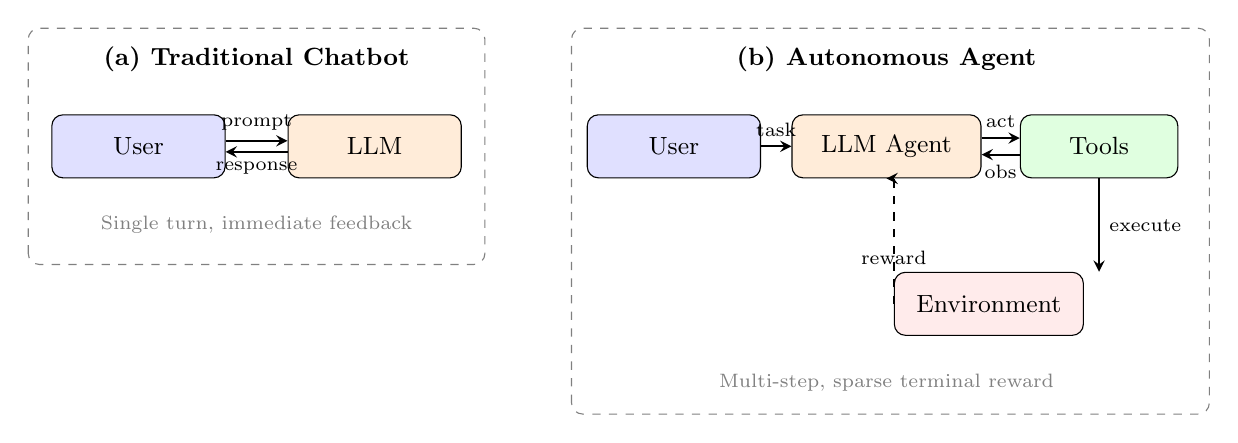
\begin{tikzpicture}[
  box/.style={draw, rounded corners, minimum width=2.2cm, minimum height=0.8cm, font=\small},
  arrow/.style={->, thick, >=stealth},
  lbl/.style={font=\scriptsize, midway, above},
  lblb/.style={font=\scriptsize, midway, below},
]
% --- (a) Chatbot ---
\node[font=\small\bfseries] at (-3.5, 2.6) {(a) Traditional Chatbot};
\node[box, fill=blue!12] (user1) at (-5, 1.5) {User};
\node[box, fill=orange!15] (llm1) at (-2, 1.5) {LLM};
\draw[arrow] ([yshift=2pt]user1.east) -- node[lbl]{prompt} ([yshift=2pt]llm1.west);
\draw[arrow] ([yshift=-2pt]llm1.west) -- node[lblb]{response} ([yshift=-2pt]user1.east);
\node[font=\scriptsize, text=gray] at (-3.5, 0.5) {Single turn, immediate feedback};
\draw[dashed, gray, rounded corners] (-6.4, 0.0) rectangle (-0.6, 3.0);

% --- (b) Autonomous Agent ---
\node[font=\small\bfseries] at (4.5, 2.6) {(b) Autonomous Agent};
\node[box, fill=blue!12] (user2) at (1.8, 1.5) {User};
\node[box, fill=orange!15, minimum width=2.4cm] (agent) at (4.5, 1.5) {LLM Agent};
\node[box, fill=green!12, minimum width=2cm] (tools) at (7.2, 1.5) {Tools};
\node[box, fill=red!8, minimum width=2.4cm] (env) at (5.8, -0.5) {Environment};

% User -> Agent
\draw[arrow] (user2.east) -- node[lbl]{task} (agent.west);
% Agent <-> Tools (bidirectional = the loop)
\draw[arrow] ([yshift=3pt]agent.east) -- node[lbl]{act} ([yshift=3pt]tools.west);
\draw[arrow] ([yshift=-3pt]tools.west) -- node[lblb]{obs} ([yshift=-3pt]agent.east);
% Tools -> Environment
\draw[arrow] (tools.south) -- node[lbl, right]{execute} (tools.south |- env.north);
% Environment -> Agent (reward)
\draw[arrow, dashed] (env.west) -- node[lblb]{reward} (agent.south -| env.west) -- (agent.south);

\node[font=\scriptsize, text=gray] at (4.5, -1.5) {Multi-step, sparse terminal reward};
\draw[dashed, gray, rounded corners] (0.5, -1.9) rectangle (8.6, 3.0);
\end{tikzpicture}
\caption{From Chatbots to Autonomous Agents: Traditional LLM chatbots operate in a single-step conversational loop with immediate human feedback. Autonomous agents plan across multiple tool interactions, receive feedback from real-world execution environments, and optimize for sparse terminal rewards (task success/failure).}
\end{figure}

The key differences that demand new RL approaches:

\begin{itemize}
  \item \textbf{Multi-step reasoning}: Agents must plan across 10--100+ tool calls, not just generate a single response.
  \item \textbf{External environment feedback}: Rewards come from real-world execution (test suites pass, web pages load, code compiles) --- not just human preference scores.
  \item \textbf{Structured actions}: Actions are not just tokens but structured outputs (JSON tool calls, API payloads, code blocks).
  \item \textbf{Long horizons with sparse rewards}: Success/failure may only be determined after many intermediate steps.
\end{itemize}

\begin{intuitionbox}[Why Standard RLHF Falls Short for Agents]
Standard RLHF (PPO/DPO) optimizes for single-turn quality: given a prompt, produce a good response. But agents must:

\begin{itemize}
  \item Decide \emph{when} to use tools vs. reason internally
  \item Recover from errors mid-trajectory (self-correction)
  \item Balance exploration (try new approaches) with exploitation (use known-good patterns)
  \item Handle partial observability (tool outputs may be incomplete or noisy)
\end{itemize}

This requires training methods that reason over \textbf{entire trajectories}, not individual turns.
\end{intuitionbox}

\section{Trajectory Buffers for LLM Agents}
\label{trajectory-buffers-for-llm-agents}

In the context of LLM agents, traditional RL replay buffers undergo a structural transformation. Instead of storing low-dimensional numerical tensors, agentic buffers --- often called \textbf{Trajectory Buffers}, \textbf{Experience Pools}, or \textbf{Memory Banks} --- manage complex textual histories, tool execution outputs, and explicit reasoning steps.

\subsection{Mathematical Structure of an LLM Agent Buffer}
\label{mathematical-structure-of-an-llm-agent-buffer}

In classic RL, a replay buffer stores a flat tuple $(s, a, r, s')$. For an LLM agent, this expands into high-dimensional tokenized text structures:

\begin{equation}
\boxed{e_t = \left( \mathcal{S}_t,\; \mathcal{A}_t,\; \mathcal{R}_t,\; \mathcal{S}_{t+1} \right)}
\end{equation}

\begin{itemize}
  \item $\mathcal{S}_t$: The \textbf{complete context state} --- system prompt, user objective, conversation history, and current environmental variables (e.g., HTML source code, directory structures, database schemas).
  \item $\mathcal{A}_t$: The agent’s \textbf{generated output}, typically composed of a Chain-of-Thought (CoT) reasoning string followed by a structured tool call: 
\begin{equation}
\mathcal{A}_t = \{\text{text}_{\text{reasoning}},\; \text{json}_{\text{tool\_call}}\}
\end{equation}
  \item $\mathcal{R}_t$: \textbf{Evaluation signals} derived from external execution environments (unit test passes, compiler flags, API response codes) or verified by an LLM-as-a-judge system.
  \item $\mathcal{S}_{t+1}$: The \textbf{updated context window}, which appends tool output text or error logs directly into the conversation history.
\end{itemize}

\begin{examplebox}[Concrete Agent Trajectory: Code Debugging]
\textbf{Step 1}: $\mathcal{S}_1$ = ``Fix the failing test in \texttt{utils.py}''\\

$\mathcal{A}_1$ = \emph{``Let me read the file first''} + \texttt{read\_file("utils.py")}\\

$\mathcal{R}_1$ = 0 (intermediate step)\\

\textbf{Step 2}: $\mathcal{S}_2$ = [previous context + file contents]\\

$\mathcal{A}_2$ = \emph{``The bug is on line 42, off-by-one error''} + \texttt{edit\_file("utils.py", ...)}\\

$\mathcal{R}_2$ = 0 (intermediate step)\\

\textbf{Step 3}: $\mathcal{S}_3$ = [previous context + edit confirmation]\\

$\mathcal{A}_3$ = \emph{``Let me verify the fix''} + \texttt{run\_tests()}\\

$\mathcal{R}_3$ = +1.0 (all tests pass --- sparse terminal reward)
\end{examplebox}

\section{Operational Paradigms}
\label{operational-paradigms}

LLM agents leverage specialized trajectory buffers through three primary optimization methodologies:

\subsection{A. Self-Correction and Thought Refinement}
\label{a.-self-correction-and-thought-refinement-star-reflexion}

Two representative methods in this category are STaR \cite{zelikman2022star} and Reflexion \cite{shinn2023reflexion}. When an agent fails a multi-step execution trace, the sub-optimal sequence is saved to the buffer. The framework later samples this trajectory and prompts the LLM to generate an explicit textual critique of its past performance: 
\begin{equation}
\text{Critique} \leftarrow \text{LLM}(\mathcal{S}_{\text{failed}},\; \mathcal{A}_{\text{failed}},\; \mathcal{R}_{=0})
\end{equation}

Once a corrected trajectory achieves a positive reward, it is moved to an optimal experience pool used to update the network weights via fine-tuning (SFT on successful trajectories) or RL (GRPO~\cite{shao2024deepseekmath} with binary pass/fail rewards).

\begin{keybox}[STaR: Self-Taught Reasoner]
\begin{enumerate}
  \item Generate reasoning traces for a batch of problems
  \item Filter: keep only traces that lead to correct answers
  \item Fine-tune the model on successful traces (SFT)
  \item Repeat: the improved model generates better traces in the next iteration
\end{enumerate}

Each iteration bootstraps the model’s reasoning ability using its own successful outputs as training data.
\end{keybox}

\begin{keybox}[Reflexion: Verbal Reinforcement Learning]
\begin{enumerate}
  \item Agent attempts a task, fails
  \item Agent generates a \textbf{verbal reflection}: ``I failed because I didn’t check the return type before calling the API''
  \item Reflection is stored in an episodic memory buffer
  \item On the next attempt, reflections are injected into the prompt as lessons learned
  \item No weight updates needed --- pure in-context learning from self-critique
\end{enumerate}
\end{keybox}

\subsection{B. Off-Policy Exploration}
\label{b.-off-policy-exploration-react-tool-use-frameworks}

This paradigm, exemplified by ReAct \cite{yao2023react} and related tool-use frameworks, involves extensive autonomous exploration. During autonomous exploration (web navigation, database querying, code generation), agents log thousands of exploratory execution paths. The trajectory buffer acts as a filter:

\begin{itemize}
  \item \textbf{Success filtering}: Only trajectories achieving the goal are kept for training.
  \item \textbf{Efficiency ranking}: Among successful traces, prefer the shortest/most efficient tool-use paths.
  \item \textbf{Diversity sampling}: Maintain a diverse set of solution strategies to prevent mode collapse.
\end{itemize}

The optimization algorithm (typically GRPO~\cite{shao2024deepseekmath} or filtered SFT) computes losses exclusively over efficient, successful trajectories while discarding meandering runs.

\subsection{C. Non-Parametric In-Context Learning (RAG over Experiences)}
\label{c.-non-parametric-in-context-learning-rag-over-experiences}

Instead of modifying neural network weights, the trajectory buffer can function as a \textbf{vector database}. Given a new user goal $\mathcal{G}_{\text{new}}$, the system retrieves the most relevant past experiences: 
\begin{equation}
\boxed{\mathcal{E}_{\text{retrieved}} = \arg\max_{e \in \mathcal{B}} \text{sim}\!\left(\text{Embed}(\mathcal{G}_{\text{new}}),\; \text{Embed}(e)\right)}
\end{equation}

The top-$k$ similar successful historical runs are injected directly into the prompt context as few-shot demonstrations. This approach:

\begin{itemize}
  \item Requires \textbf{zero training} --- pure retrieval-augmented generation
  \item Adapts instantly to new tasks if similar experiences exist in the buffer
  \item Scales with buffer size (more experiences = better coverage)
  \item Complements parametric learning (use retrieval for rare cases, weights for common patterns)
\end{itemize}

\section{Paradigm Comparison}
\label{paradigm-comparison}

\begin{table}[ht!]
\centering
\caption{Traditional RL Buffers vs. LLM Agent Buffers}
\begin{tabular}{@{}lp{5cm}p{8cm}@{}}
\toprule
\textbf{Feature} & \textbf{Traditional RL Buffer} & \textbf{LLM Agent Buffer} \\
\midrule
\textbf{Data Format} & Continuous vectors / tensors & Tokenized text, JSON, code blocks, tool outputs \\
\textbf{Data Volume} & Massive ($10^5$--$10^7$ items) & Small to medium ($10^3$--$10^5$ traces) \\
\textbf{Primary Goal} & Breaking data correlation & Providing reasoning demonstrations \\
\textbf{Sampling} & Random uniform / PER & Semantic retrieval / success priority / diversity \\
\textbf{State Size} & Fixed (e.g., 84$\times$84 pixels) & Variable (1K--128K tokens per state) \\
\textbf{Action Space} & Discrete/continuous vectors & Structured text (reasoning + tool calls) \\
\textbf{Reward Source} & Environment simulator & External execution / LLM judge / unit tests \\
\bottomrule
\end{tabular}
\end{table}

\section{Major Techniques in Agentic RL}
\label{major-techniques-in-agentic-rl}

\begin{table}[ht!]
\centering
\caption{Key methods for training LLM agents with RL.}
\begin{tabular}{@{}lp{5cm}p{8cm}@{}}
\toprule
\textbf{Method} & \textbf{Type} & \textbf{Key Idea} \\
\midrule
\textbf{STaR}~\cite{zelikman2022star} & Iterative SFT & Bootstrap reasoning by fine-tuning on own successful traces \\
\textbf{Reflexion}~\cite{shinn2023reflexion} & In-context RL & Verbal self-critique stored as episodic memory; no weight updates \\
\textbf{ReAct}~\cite{yao2023react} & Prompting & Interleave reasoning (``think'') and acting (``tool call'') in a single generation \\
\textbf{LATS}~\cite{zhou2024lats} & Tree search & Monte Carlo Tree Search over action sequences; backpropagate rewards \\
\textbf{AgentQ}~\cite{putta2024agentq} & Off-policy RL & DPO on agent trajectories with AI-generated preference pairs \\
\textbf{OpenHands}~\cite{wang2024openhands} & GRPO & Group-relative optimization with execution-based rewards (tests pass/fail) \\
\textbf{Voyager}~\cite{wang2023voyager} & Skill library & Successful code snippets stored and retrieved for compositional reuse \\
\textbf{RLEF}~\cite{le2024rlef} & Online RL & RL from Execution Feedback --- binary reward from code/test execution \\
\bottomrule
\end{tabular}
\end{table}

\subsection{STaR: Self-Taught Reasoner (Detailed)}
\label{star-self-taught-reasoner-detailed}

STaR~\cite{zelikman2022star} is an \textbf{iterative self-improvement} method that bootstraps reasoning capabilities without external reward models. The core insight: if the model can occasionally solve a problem correctly, it can learn from its own successes.

\textbf{Algorithm}:

\begin{enumerate}
  \item \textbf{Generate}: For each problem $x_i$ in dataset $\mathcal{D}$, sample a reasoning trace $z_i \sim \pi_\theta(\cdot | x_i)$ followed by an answer $\hat{y}_i$.
  \item \textbf{Filter}: Keep only traces where $\hat{y}_i = y_i^*$ (correct answer). Define success set $\mathcal{D}_{\text{pass}} = \{(x_i, z_i, y_i^*) : \hat{y}_i = y_i^*\}$.
  \item \textbf{Rationalization} (key innovation): For problems where the model failed, generate a ``rationalization'' --- a trace conditioned on the correct answer: $z_i^{\text{rat}} \sim \pi_\theta(\cdot | x_i, y_i^*)$. This teaches the model to reason \emph{backward} from solutions.
  \item \textbf{Fine-tune}: Update $\theta$ via SFT on $\mathcal{D}_{\text{pass}} \cup \mathcal{D}_{\text{rationalized}}$.
  \item \textbf{Iterate}: Repeat from step 1 with the improved model.
\end{enumerate}

\begin{equation}
\boxed{\theta_{k+1} = \arg\min_\theta -\sum_{(x,z,y) \in \mathcal{D}_k^+} \log \pi_\theta(z, y | x)}
\end{equation}

\textbf{Convergence dynamics}: Each iteration $k$ increases the model’s solve rate $p_k$. If $p_0 = 0.3$ (solves 30\% of problems), after rationalization + SFT, $p_1 \approx 0.5$. Typically converges in 3--5 iterations to $p \approx 0.7$--$0.9$.

\begin{examplebox}[STaR Rationalization Prompt]
\begin{lstlisting}[style=pythonstyle]
# Standard generation (Step 1):
PROMPT = """Solve the following problem step by step.
Problem: A store has 45 apples. It sells 3/5 of them. How many remain?
Let's think step by step:"""

# Rationalization prompt (Step 3 - conditioned on correct answer):
PROMPT_RATIONALIZE = """Solve the following problem step by step.
The correct answer is 18.
Problem: A store has 45 apples. It sells 3/5 of them. How many remain?
Let's think step by step to arrive at 18:"""

# Agent variant (code task with error conditioning):
PROMPT_AGENT_RATIONALIZE = """The following code task failed with the error below.
Generate a correct solution step by step.

Task: Implement binary search that handles duplicates.
Previous error: IndexError: list index out of range (line 12)
Correct behavior: Return leftmost index of target.

Let me fix this by reasoning about the boundary conditions:"""
\end{lstlisting}
\end{examplebox}

\begin{intuitionbox}[STaR Variants for Agents]
\begin{itemize}
  \item \textbf{Quiet-STaR}~\cite{zelikman2024quietstar}: Inserts ``thinking tokens'' between every token of generation. The model learns to reason \emph{implicitly} without explicit CoT prompting. Training objective: predict next tokens better when thinking tokens are included.
  \item \textbf{STaR for Code Agents}: Replace answer verification with test execution. ``Correct'' = all tests pass. Rationalization = generate a new approach conditioned on the error message.
  \item \textbf{V-STaR}~\cite{hosseini2024vstar}: Adds a verifier model trained on $(z, y, \text{correct/incorrect})$ triples. The verifier provides process-level supervision, filtering bad reasoning traces that accidentally reach correct answers.
\end{itemize}
\end{intuitionbox}

\subsection{Reflexion: Verbal Reinforcement Learning (Detailed)}
\label{reflexion-verbal-reinforcement-learning-detailed}

Reflexion~\cite{shinn2023reflexion} introduces a radical paradigm: \textbf{RL without weight updates}. Instead of gradient-based learning, the agent improves through natural-language self-critique stored in an episodic memory.

\textbf{Full Architecture}:

\begin{enumerate}
  \item \textbf{Actor}: The LLM agent $\pi$ that executes actions in the environment.
  \item \textbf{Evaluator}: A binary signal (task success/failure) or a scalar heuristic (e.g., number of test cases passed).
  \item \textbf{Self-Reflection Generator}: Given the failed trajectory $\tau_{\text{fail}}$ and environment feedback, generates a natural-language reflection $r_{\text{text}}$: 
\begin{equation}
r_{\text{text}} = \text{LLM}_{\text{reflect}}\!\left(\tau_{\text{fail}}, \text{feedback}, \text{task}\right)
\end{equation}
  \item \textbf{Episodic Memory}: A sliding window buffer $\mathcal{M} = [r_1, r_2, \ldots, r_m]$ of past reflections (typically $m \leq 3$ to fit in context).
  \item \textbf{Retry Loop}: On the next attempt, reflections are injected into the prompt: 
\begin{equation}
a_{t+1} \sim \pi\!\left(\cdot\; |\; \text{task},\; \mathcal{M},\; \text{current\_state}\right)
\end{equation}
\end{enumerate}

\textbf{Example reflection}: \emph{``In my previous attempt, I called the search API before validating the input format, which caused a 400 error. Next time, I should validate the JSON schema first, then make the API call.''}

\begin{examplebox}[Reflexion: Agent Prompt with Injected Memory]
\begin{lstlisting}[style=pythonstyle]
# === ATTEMPT 2 PROMPT (after first failure) ===

SYSTEM = """You are a coding agent. You can run bash commands and edit files.
Complete the task below. Learn from your previous reflections."""

USER = """Task: Fix the failing test in auth_service.py

=== REFLECTIONS FROM PREVIOUS ATTEMPTS ===
[Attempt 1 reflection]: I tried to modify the authenticate() function
directly but forgot that it depends on token_validator(). The test
failed because token_validator() was still returning the old format.
I should trace the dependency chain FIRST: check what authenticate()
calls, then fix the root cause (token_validator), not the symptom.
=== END REFLECTIONS ===

The repository is in /workspace/. The failing test is:
  test_auth.py::test_expired_token_returns_401

Begin by reading the relevant files, then fix the issue."""
\end{lstlisting}
\end{examplebox}

\textbf{Strengths and Limitations}:

{\small
\begin{tabular}{@{}p{7.5cm}p{7.5cm}@{}}
\toprule
\textbf{Strengths} & \textbf{Limitations} \\
\midrule
Zero gradient computation; works with frozen API models (GPT-4) & Limited to context window; can’t accumulate infinite knowledge \\
Fast iteration (seconds per retry vs. hours for RL training) & No generalization to unseen tasks (memory is task-specific) \\
Interpretable: human-readable self-corrections & Relies on the model’s existing ability to identify errors \\
Composes with any base agent architecture & Degrades when base model is too weak to generate useful critiques \\
\bottomrule
\end{tabular}
}

\subsection{ReAct: Reasoning + Acting (Detailed)}
\label{react-reasoning-acting-detailed}

ReAct~\cite{yao2023react} establishes the dominant prompting paradigm for tool-using agents by \textbf{interleaving explicit reasoning steps with environment actions} in a single generation stream.

\begin{examplebox}[ReAct System Prompt (Typical)]
\begin{lstlisting}[style=pythonstyle]
SYSTEM = """You are a research assistant with access to the following tools:
- search(query): Search the web for information
- lookup(term): Look up a term on the current Wikipedia page
- finish(answer): Submit your final answer

Solve the user's question by interleaving Thought and Action steps.
Format:
  Thought: <your reasoning about what to do next>
  Action: <tool_name>(arguments)

You will receive an Observation after each Action. Use it to plan
your next step. Continue until you can provide a final answer.

Rules:
- Always think before acting
- Never guess - verify with tools
- Use finish() only when you are confident in your answer"""

USER = "Who was the president of the US when the iPhone was released?"
\end{lstlisting}
\end{examplebox}

\textbf{Generation format}:

\begin{examplebox}[ReAct Trace Format]
\begin{lstlisting}[style=pythonstyle]
Thought: I need to find when the iPhone was released, then determine
who was president at that time. Let me search for the release date.
Action: search("iPhone original release date")
Observation: The original iPhone was released on June 29, 2007.
Thought: The iPhone came out June 2007. Now I need to find who was
the US president in June 2007.
Action: lookup("President of the United States in 2007")
Observation: George W. Bush served as the 43rd president from
January 20, 2001 to January 20, 2009.
Thought: George W. Bush was president from 2001-2009, which covers
June 2007 when the iPhone was released. I have my answer.
Action: finish("George W. Bush was the US president when the iPhone
was released on June 29, 2007.")
\end{lstlisting}
\end{examplebox}

\textbf{Formal definition}: A ReAct trajectory is $\tau = (t_1, a_1, o_1, t_2, a_2, o_2, \ldots)$ where:

\begin{itemize}
  \item $t_i$: Thought (internal reasoning, not executed)
  \item $a_i$: Action (tool call, executed in environment)
  \item $o_i$: Observation (environment response, appended to context)
\end{itemize}

\textbf{Why it works}: Thoughts create an ``inner monologue'' that helps the model plan before acting, reducing impulsive tool calls. The explicit reasoning trace also makes the agent’s decision process \textbf{auditable} and \textbf{debuggable}.

\textbf{Training ReAct agents with RL}:

\begin{itemize}
  \item \textbf{Action-level rewards}: Only actions receive reward signals (thoughts are auxiliary).
  \item \textbf{Thought quality}: Implicitly optimized --- better thoughts $\rightarrow$ better actions $\rightarrow$ higher rewards.
  \item \textbf{Format enforcement}: Include format penalties in the reward for malformed actions (missing JSON, hallucinated tools).
  \item \textbf{RL objective}: $r(\tau) = r_{\text{task}} - \lambda_{\text{format}} \cdot \text{format\_violations} - \lambda_{\text{length}} \cdot \text{num\_steps}$
\end{itemize}

\subsection{LATS: Language Agent Tree Search (Detailed)}
\label{lats-language-agent-tree-search-detailed}

LATS~\cite{zhou2024lats} applies \textbf{Monte Carlo Tree Search (MCTS)} to LLM agent action selection, trading inference compute for significantly better trajectories.

\textbf{Algorithm (adapted for LLM agents)}:

\begin{enumerate}
  \item \textbf{Selection}: Starting from root (initial state), traverse the tree using UCB1: 
\begin{equation}
\text{UCB}(s, a) = \bar{Q}(s, a) + c \sqrt{\frac{\ln N(s)}{N(s, a)}}
\end{equation}
 where $\bar{Q}$ = average reward of subtree, $N$ = visit counts, $c$ = exploration constant.
  \item \textbf{Expansion}: At a leaf node, generate $k$ candidate actions via LLM sampling (temperature $> 0$): $\{a_1, \ldots, a_k\} \sim \pi_\theta(\cdot | s_{\text{leaf}})$
  \item \textbf{Simulation}: For each candidate, execute the action in the environment and continue with a fast rollout policy (greedy decoding) until terminal state or depth limit.
  \item \textbf{Backpropagation}: Propagate the terminal reward up through all ancestor nodes, updating $\bar{Q}$ and $N$ counts.
  \item \textbf{Repeat}: Run steps 1--4 for a fixed computation budget (e.g., 50--200 iterations).
  \item \textbf{Action selection}: Choose the most-visited child of the root.
\end{enumerate}

\textbf{LLM-specific adaptations}:

\begin{itemize}
  \item \textbf{Value function}: Use a separate LLM call to estimate state value: ``On a scale of 0--1, how likely is this state to lead to task success?''
  \item \textbf{Reflection-based pruning}: When a branch fails, generate a reflection and prune similar branches.
  \item \textbf{Caching}: Store LLM outputs at each node to avoid redundant generation during backtracking.
  \item \textbf{Depth budget}: Limit tree depth to 10--20 steps (agents rarely need more).
\end{itemize}

\textbf{Performance}: On WebShop (web navigation), LATS achieves 75\% success vs. ReAct’s 40\%. On HumanEval (code), pass@1 improves from 68\% $\rightarrow$ 94\% with tree search. The cost: 10--50$\times$ more inference FLOPs per task.

\begin{examplebox}[LATS Prompts: Value Estimation and Node Expansion]
\begin{lstlisting}[style=pythonstyle]
# === VALUE ESTIMATION PROMPT (used during simulation) ===
VALUE_PROMPT = """You are evaluating an agent's progress on a task.

Task: Book a flight from NYC to London for under \$500, departing Dec 15.

Current state (after 3 actions):
- Searched flights on Kayak: found 12 results
- Filtered by price < \$500: 4 options remain
- Clicked on British Airways \$489 option: viewing details page

On a scale of 0.0 to 1.0, how likely is the agent to successfully
complete the task from this state? Consider:
- How close is the agent to the goal?
- Are there remaining obstacles (payment, seat selection)?
- Has the agent made any errors that need correction?

Score: """  # Model outputs e.g. "0.75"

# === NODE EXPANSION PROMPT (generating candidate actions) ===
EXPAND_PROMPT = """You are a web navigation agent. Given the current
page state, propose 3 DIFFERENT next actions to try.

Current page: British Airways booking - flight details
  Price: \$489 | Departure: Dec 15 8:30am | Arrival: Dec 15 8:45pm
  [Button: Select] [Button: Back to results] [Link: Fare rules]

Generate 3 diverse candidate actions (explore different strategies):
Action 1:"""  # Model generates 3 options for tree expansion
\end{lstlisting}
\end{examplebox}

\subsection{AgentQ: DPO on Agent Trajectories (Detailed)}
\label{agentq-dpo-on-agent-trajectories-detailed}

AgentQ~\cite{putta2024agentq} bridges \textbf{offline preference learning (DPO)} with \textbf{online agent execution} by automatically generating preference pairs from trajectory outcomes.

\textbf{Pipeline}:

\begin{enumerate}
  \item \textbf{Rollout}: Execute $N$ trajectories per task using the current policy $\pi_\theta$.
  \item \textbf{Evaluate}: Score each trajectory with execution-based reward (binary pass/fail or scalar metric).
  \item \textbf{Pair construction}: For each task, construct preference pairs: 
\begin{equation}
(\tau_w, \tau_l) \text{ where } r(\tau_w) > r(\tau_l)
\end{equation}
 Among trajectories for the same task, the one with highest reward = chosen; lowest = rejected.
  \item \textbf{DPO update}: Apply standard DPO loss over trajectory-level log-probabilities: 
\begin{equation}
\mathcal{L}_{\text{AgentQ}} = -\log \sigma\!\left(\beta \left[\log\frac{\pi_\theta(\tau_w)}{\pi_{\text{ref}}(\tau_w)} - \log\frac{\pi_\theta(\tau_l)}{\pi_{\text{ref}}(\tau_l)}\right]\right)
\end{equation}
  \item \textbf{Iterate}: Updated $\pi_\theta$ generates new (better) trajectories in the next round.
\end{enumerate}

\textbf{Key design choices}:

\begin{itemize}
  \item \textbf{MCTS-guided exploration}: Use LATS during rollout phase to generate diverse, high-quality trajectories (better training data).
  \item \textbf{Step-level DPO}: Instead of comparing full trajectories, compare at the \emph{action level} --- given the same prefix, which next action leads to success?
  \item \textbf{Self-play improvement}: Each DPO iteration produces a better policy that generates better trajectories that produce better training pairs --- a virtuous cycle.
\end{itemize}

\textbf{Results}: On WebShop, AgentQ achieves absolute 50\% $\rightarrow$ 82\% success rate improvement over the base policy in 3 DPO iterations.

\subsection{Voyager: Lifelong Learning via Skill Libraries (Detailed)}
\label{voyager-lifelong-learning-via-skill-libraries-detailed}

Voyager~\cite{wang2023voyager} introduces \textbf{compositional skill accumulation} --- the agent builds a growing library of reusable code functions that serve as high-level actions.

\textbf{Architecture}:

\begin{enumerate}
  \item \textbf{Automatic Curriculum}: An LLM proposes progressively harder tasks based on the agent’s current skill inventory: ``You can now mine wood and craft planks. Next challenge: build a crafting table.''
  \item \textbf{Skill Generation}: For each task, the agent writes a JavaScript function (executable code) that solves it: 
\begin{equation}
\text{skill}_i = \text{LLM}(\text{task}_i, \text{environment\_docs}, \text{error\_feedback})
\end{equation}
  \item \textbf{Verification}: Execute the code in the environment. If it succeeds, add to the skill library. If not, iterate with error feedback (up to 5 retries).
  \item \textbf{Skill Library} (vector DB): Each verified skill stored with:

\begin{itemize}
  \item Function signature + docstring (for retrieval)
  \item Embedding of the task description (for semantic search)
  \item Dependencies (which other skills it calls)
\end{itemize}
  \item \textbf{Retrieval + Composition}: For new tasks, retrieve the top-$k$ most relevant skills and compose them: 
\begin{equation}
\text{solution} = \text{LLM}(\text{new\_task}, \text{retrieve}(\text{skill\_library}, k{=}5))
\end{equation}
\end{enumerate}

\textbf{Key insight}: Skills are \textbf{compositional} --- complex behaviors emerge from combining simple verified functions. The agent never forgets (library is persistent) and improves monotonically (only verified skills are added).

\begin{examplebox}[Voyager: Curriculum and Skill Generation Prompts]
\begin{lstlisting}[style=pythonstyle]
# === AUTOMATIC CURRICULUM PROMPT ===
CURRICULUM_PROMPT = """You are a curriculum designer for an AI agent.

Agent's current skill inventory:
- mine_wood(): Mines nearby oak/birch trees
- craft_planks(): Converts logs to planks
- craft_sticks(): Converts planks to sticks
- mine_stone(): Mines stone with wooden pickaxe

Propose the next task that:
1. Builds on existing skills (reachable from current abilities)
2. Introduces exactly ONE new concept or challenge
3. Is concrete and verifiable (clear success condition)

Next task proposal:"""
# Output: "Craft a furnace (requires 8 cobblestone blocks arranged
#          in a square). You already know mine_stone()."

# === SKILL GENERATION PROMPT ===
SKILL_GEN_PROMPT = """Write a JavaScript function to accomplish this task
in Minecraft. Use the bot API (bot.dig, bot.craft, bot.equip, etc.)

Task: Smelt 5 iron ingots using a furnace.
Prerequisites available: mine_stone(), craft_furnace(), mine_iron_ore()

Error from previous attempt: "Cannot smelt without fuel in furnace"

Write the corrected function:
async function smeltIronIngots(bot, count=5) {"""
\end{lstlisting}
\end{examplebox}

\subsection{RLEF: RL from Execution Feedback (Detailed)}
\label{rlef-rl-from-execution-feedback-detailed}

RLEF~\cite{le2024rlef} applies \textbf{online RL with deterministic execution-based rewards} to code generation agents, establishing the simplest effective paradigm for agentic training.

\textbf{Training loop}:

\begin{enumerate}
  \item \textbf{Sample task}: Draw a coding problem with test cases $(x, \text{tests})$ from the training set.
  \item \textbf{Generate}: The agent produces a solution trajectory (reading files, writing code, running tests) using the current policy $\pi_\theta$.
  \item \textbf{Execute}: Run the test suite in a sandboxed environment. Reward: 
\begin{equation}
r = \frac{\text{\# tests passed}}{\text{\# total tests}} \in [0, 1]
\end{equation}
  \item \textbf{Update}: Apply GRPO/PPO using $r$ as the reward signal.
  \item \textbf{Repeat}: Thousands of iterations with fresh tasks.
\end{enumerate}

\textbf{Why execution feedback is ideal for RL}:

\begin{itemize}
  \item \textbf{Zero noise}: Unlike human preferences, test results are deterministic. Same code $\rightarrow$ same reward every time. This eliminates reward noise that destabilizes RL training.
  \item \textbf{Infinite scale}: Can generate unlimited tasks programmatically (random algorithms, API integration tests, data transformations).
  \item \textbf{No reward hacking}: Unlike learned reward models, a test suite can’t be ``fooled'' (assuming tests are well-written). The agent must actually solve the problem.
  \item \textbf{Dense signal}: Partial test passage ($r = 0.6$) provides richer gradient than binary pass/fail.
\end{itemize}

\subsection{OpenHands / SWE-Agent: GRPO for Software Engineering}
\label{openhands-swe-agent-grpo-for-software-engineering}

OpenHands~\cite{wang2024openhands} and SWE-Agent~\cite{yang2024sweagent} apply GRPO to train agents that autonomously resolve GitHub issues --- reading code, writing patches, and running test suites.

\textbf{Training specifics}:

\begin{itemize}
  \item \textbf{Environment}: Docker container with full repo, test suite, and developer tools (git, grep, lint).
  \item \textbf{Action space}: Bash commands, file edits, git operations, test execution.
  \item \textbf{Trajectory length}: 15--50 actions typical for resolving a GitHub issue.
  \item \textbf{Reward}: Binary --- does the generated patch pass the issue’s regression tests?
  \item \textbf{Group size}: $N = 8$--$16$ trajectories per issue for GRPO normalization.
  \item \textbf{Curriculum}: Start with issues labeled ``good first issue'', progress to complex multi-file refactors.
\end{itemize}

\textbf{State-of-the-art results}: SWE-bench Verified: 30\% $\rightarrow$ 55\% resolve rate after RL training (vs. SFT-only baseline).

\begin{examplebox}[OpenHands / SWE-Agent: System Prompt]
\begin{lstlisting}[style=pythonstyle]
SYSTEM = """You are an autonomous software engineer. You are given a
GitHub issue to resolve. You have access to the full repository in
/workspace/ and can execute any bash command.

AVAILABLE COMMANDS:
- bash(command): Execute a shell command
- edit(file, start_line, end_line, new_content): Edit a file
- search(pattern, path): Search for text in files
- submit(): Submit your patch when done

WORKFLOW:
1. Read the issue carefully and understand the expected behavior
2. Explore the codebase to find relevant files
3. Reproduce the bug (write/run a test that fails)
4. Implement the fix
5. Verify the fix (run the test again - must pass)
6. Run the full test suite to check for regressions
7. Submit when all tests pass

RULES:
- Do NOT modify test files unless the issue explicitly asks for it
- Prefer minimal, targeted changes over large refactors
- Always verify your fix before submitting"""

USER = """GitHub Issue #4521: `DataFrame.merge()` silently drops
rows when `on` column contains NaN values.

Expected: NaN keys should be preserved (matched with other NaN rows)
Actual: Rows with NaN keys are dropped entirely

Repository: /workspace/pandas-dev/pandas/"""
\end{lstlisting}
\end{examplebox}

\begin{intuitionbox}[The Future: RL + Agents]
The field is converging on a pattern: \textbf{online RL with execution-based rewards} applied to multi-step agent trajectories. Key trends:

\begin{itemize}
  \item GRPO/PPO with binary pass/fail rewards from code execution or tool success
  \item Curriculum learning: start with easy tasks, progressively increase difficulty
  \item Trajectory-level optimization (not token-level) --- reward only at the end of a multi-step sequence
  \item Hybrid approaches: use retrieval (non-parametric) for rare tasks + RL (parametric) for common ones
  \item Scaling law: more compute at inference (search/retry) often beats more training compute
\end{itemize}
\end{intuitionbox}

\newpage
\section{Use Case: Agentic RL for a Productivity Co-pilot}
\label{use-case-agentic-rl-for-a-productivity-co-pilot}

This section provides a complete blueprint for applying agentic RL techniques to train an LLM-based co-pilot that operates across a productivity application suite (documents, spreadsheets, presentations, email, messaging, cloud storage).

\subsection{Architecture Overview}
\label{architecture-overview}

\begin{figure}[ht!]
\centering

\includegraphics[width=0.85\textwidth]{figures/fig_043_fig43.png}
\caption{Productivity co-pilot architecture: the LLM agent (with RL policy $\pi_\theta$) receives user intents and interacts with multiple application APIs. A reward signal based on task success, user feedback, and efficiency metrics drives policy improvement.}
\end{figure}

\subsection{Formal MDP Definition for a Productivity Co-pilot}
\label{formal-mdp-definition-for-a-productivity-co-pilot}

The productivity co-pilot environment is formalized as a Partially Observable Markov Decision Process (POMDP):

\begin{equation}
\boxed{\mathcal{M} = \langle \mathcal{S}, \mathcal{A}, \mathcal{T}, \mathcal{R}, \Omega, \mathcal{O}, \gamma \rangle}
\end{equation}

\begin{itemize}
  \item $\mathcal{S}$: \textbf{State space} --- Full workspace environment state: document contents, email threads, calendar events, file system, user permissions. \emph{Not fully observable}: agent sees only what API queries return.
  \item $\mathcal{A}$: \textbf{Action space} --- Structured API calls (see below). Each action is a JSON object specifying the target app, operation, and parameters.
  \item $\mathcal{T}$: \textbf{Transition function} --- Deterministic for most operations (write to document $\rightarrow$ document updated), but stochastic for network-dependent actions (email delivery time, Teams availability).
  \item $\mathcal{R}$: \textbf{Reward function} --- Multi-component (see Reward Design section).
  \item $\Omega$: \textbf{Observation space} --- API responses, rendered document views, error messages.
  \item $\mathcal{O}$: \textbf{Observation function} --- Maps state to observation (API response formatting, truncation for context window limits).
  \item $\gamma = 0.99$: Discount factor (long horizons, 10--50 steps typical).
\end{itemize}

\begin{examplebox}[Concrete Example: ``Summarize last week’s Project Alpha emails and create a status slide'']
Below we trace a full episode through the POMDP, mapping each formal element to a concrete realization.

\textbf{User request}: ``Summarize the key decisions from last week’s Project Alpha emails and add a status update slide to the team deck.''

\begin{tabular}{@{}lp{11cm}@{}}
\toprule
\textbf{Symbol} & \textbf{Concrete Realization} \\
\midrule
$s_0$ & \emph{True state}: 47 emails in inbox mentioning ``Project Alpha'' from last 7 days; PowerPoint file ``Q3\_Status.pptx'' on SharePoint with 12 slides; user has edit permissions. \\
$o_0$ & \emph{Agent observes}: User request text + system prompt. Agent has \emph{no knowledge} of email count or deck contents yet. \\
$a_1$ & \verb|outlook.search({query: "Project Alpha", last\_7\_days: true})| \\
$\mathcal{T}(s_0, a_1)$ & $s_1$: System retrieves 47 matching emails (deterministic). \\
$o_1$ & API returns top 10 email subjects + senders + timestamps (truncated due to context limits --- $\mathcal{O}$ in action). \\
$a_2$ & \verb|outlook.read({ids: [top\_5\_thread\_ids]})| --- Agent picks the most relevant threads. \\
$o_2$ & Full body text of 5 email threads ($\sim$8K tokens after $\mathcal{O}$ truncation). \\
$a_3$ & \emph{Internal reasoning action}: Agent synthesizes key decisions: (1) deadline moved to Nov 15, (2) budget approved, (3) vendor selected. \\
$a_4$ & \verb|sharepoint.read({file: "Q3\_Status.pptx", slides: "last"})| --- Check current last slide. \\
$o_4$ & Last slide is ``Q2 Summary'' (slide 12). Agent decides to add slide 13. \\
$a_5$ & \verb|powerpoint.add\_slide({file: "Q3\_Status.pptx", position: 13,| \texttt{layout: "Title and Content", title: "Project Alpha --- Week 42 Status",} \verb|content: "Key decisions: 1) Deadline: Nov 15..."})| \\
$\mathcal{T}(s_4, a_5)$ & $s_5$: Slide added to deck (deterministic). \\
$o_5$ & API returns \verb|{success: true, slide\_id: 13}|. \\
$R(s_5)$ & Reward components: \textbf{+0.4} task completion (slide created), \textbf{+0.3} information quality (correct decisions extracted), \textbf{+0.2} format compliance (proper layout used), \textbf{+0.05} efficiency (5 actions, no errors), \textbf{-0.0} safety penalty. \textbf{Total: 0.95}. \\
\bottomrule
\end{tabular}

\textbf{Key POMDP aspects illustrated}:

\begin{itemize}
  \item \textbf{Partial observability}: At $t=0$, the agent doesn’t know how many emails exist or what the deck contains --- it must query to discover the state.
  \item \textbf{Observation function $\mathcal{O}$}: The API returns truncated results (top 10 of 47 emails) due to context window limits. The agent sees a \emph{projection} of the true state.
  \item \textbf{Stochastic transitions}: If the agent had tried \texttt{teams.send\_message()} instead, delivery timing would be uncertain (recipient online/offline).
  \item \textbf{Multi-step planning}: The agent must chain 5 actions across 2 applications, maintaining coherence between the email summary and the slide content.
  \item \textbf{Discount $\gamma=0.99$}: With 5 steps, discounting is minimal ($0.99^5 = 0.95$), but for 50-step tasks it matters --- encouraging efficient solutions.
\end{itemize}
\end{examplebox}

\subsection{Action Space Design}
\label{action-space-design}

The action space must be \textbf{structured, type-safe, and composable}:

\begin{examplebox}[Productivity Co-pilot Action Schema]
\begin{lstlisting}[style=pythonstyle]
{
  "action_type": "api_call",
  "target_app": "outlook | excel | word | powerpoint | teams | sharepoint",
  "operation": "read | write | search | create | delete | modify",
  "parameters": {
    "endpoint": "/me/messages?$filter=subject eq 'Project X'",
    "body": { ... },             // For write operations
    "options": { "top": 10 }     // Pagination, filtering
  },
  "reasoning": "I need to find relevant emails before summarizing"
}
\end{lstlisting}
\end{examplebox}

\textbf{Action taxonomy by application}:

\begin{tabular}{@{}lp{5cm}p{8cm}@{}}
\toprule
\textbf{App} & \textbf{Complexity} & \textbf{Key Actions} \\
\midrule
\textbf{Outlook} & Medium & \texttt{search}, \texttt{read}, \texttt{draft}, \texttt{send}, \texttt{move}, \texttt{flag}, \texttt{create\_rule} \\
\textbf{Excel} & High & \texttt{read\_range}, \texttt{write\_range}, \texttt{insert\_formula}, \texttt{create\_chart}, \texttt{pivot\_table}, \texttt{run\_macro} \\
\textbf{Word} & Medium & \texttt{read\_paragraphs}, \texttt{insert\_text}, \texttt{format\_section}, \texttt{find\_replace}, \texttt{insert\_table} \\
\textbf{PowerPoint} & Medium & \texttt{add\_slide}, \texttt{insert\_shape}, \texttt{set\_text}, \texttt{set\_layout}, \texttt{add\_image}, \texttt{apply\_theme} \\
\textbf{Teams} & Low & \texttt{send\_message}, \texttt{create\_meeting}, \texttt{search\_chat}, \texttt{add\_members}, \texttt{post\_to\_channel} \\
\textbf{SharePoint} & Medium & \texttt{list\_files}, \texttt{upload}, \texttt{download}, \texttt{search}, \texttt{create\_page}, \texttt{set\_permissions} \\
\bottomrule
\end{tabular}

\subsection{State Representation}
\label{state-representation}

The agent’s observation (context window) at each step:

\begin{equation}
o_t = [\text{system\_prompt};\; \text{user\_intent};\; \text{tool\_history}_{1:t-1};\; \text{current\_result}_t]
\end{equation}

\textbf{Context budget management} (critical for 128K window):

\begin{itemize}
  \item \textbf{System prompt}: 2K tokens (capabilities, safety rules, output format)
  \item \textbf{User intent + conversation}: 4K tokens
  \item \textbf{Tool history} (sliding window): Last 8--12 actions + observations, summarizing older ones. Total: 80K tokens max.
  \item \textbf{Current observation}: Up to 32K tokens (large spreadsheets, email threads)
  \item \textbf{Reserve}: 10K tokens for agent’s reasoning + next action generation
\end{itemize}

\textbf{State compression strategies}:

\begin{itemize}
  \item \textbf{Selective inclusion}: Only include API responses relevant to the current sub-goal (use an auxiliary ``relevance scorer'').
  \item \textbf{Structured summaries}: Represent large spreadsheets as schema + sample rows rather than full data.
  \item \textbf{Hierarchical memory}: Store full trajectory externally; inject compressed summaries into context.
\end{itemize}

\subsection{Reward Design: Multi-Objective Signal}
\label{reward-design-multi-objective-signal}

The reward function for a productivity co-pilot must balance multiple objectives:

\begin{equation}
\boxed{R(\tau) = \alpha_1 R_{\text{task}} + \alpha_2 R_{\text{quality}} + \alpha_3 R_{\text{efficiency}} + \alpha_4 R_{\text{safety}} + \alpha_5 R_{\text{user}}}
\end{equation}

\begin{table}[ht!]
\centering
\caption{Reward components for productivity co-pilot training.}
\begin{tabular}{@{}lp{3.5cm}p{3.5cm}p{6cm}@{}}
\toprule
\textbf{Component} & \textbf{Weight} & \textbf{Signal Type} & \textbf{Definition} \\
\midrule
$R_{\text{task}}$ & 0.40 & Binary/scalar & Task completed successfully (email sent, document created, formula correct) \\
$R_{\text{quality}}$ & 0.25 & LLM judge & Output quality: formatting, clarity, correctness of content \\
$R_{\text{efficiency}}$ & 0.15 & Scalar & Penalty for excessive steps: $-0.02 \times (\text{num\_steps} - \text{optimal\_steps})$ \\
$R_{\text{safety}}$ & 0.15 & Binary & No unsafe actions (delete without confirmation, send to wrong recipient, permission violations). $R_{\text{safety}} = 0$ if any violation. \\
$R_{\text{user}}$ & 0.05 & Sparse & Explicit user feedback (thumbs up/down) when available \\
\bottomrule
\end{tabular}
\end{table}

\textbf{Intermediate rewards (dense signal)}:

\begin{itemize}
  \item Successful API call (200 response): +0.05
  \item Correct information retrieval (verified by downstream use): +0.10
  \item Recovers from error gracefully (retries with corrected params): +0.08
  \item API error (4xx/5xx): --0.03
  \item Repeated identical action (loop detection): --0.10
  \item Asks clarifying question when intent is genuinely ambiguous: +0.05
\end{itemize}

\subsection{Training Pipeline: End-to-End}
\label{training-pipeline-end-to-end}

\begin{keybox}[Productivity Co-pilot RL Training Pipeline]
\textbf{Phase 1: Supervised Fine-Tuning (Foundation)}

\begin{enumerate}
  \item Collect 50K--200K human-demonstrated trajectories of productivity tasks (via telemetry, annotators, or synthetic generation).
  \item SFT the base LLM on (instruction, trajectory) pairs with ReAct format.
  \item Validate: agent should achieve 40--60\% task completion on held-out tasks.
\end{enumerate}

\textbf{Phase 2: Simulated Environment Construction}

\begin{enumerate}
  \item Build a \textbf{sandbox environment} with mocked API endpoints, synthetic mailboxes, documents, and calendars.
  \item Each ``user'' has a realistic profile: 500+ emails, 20+ documents, calendar events, Teams channels.
  \item Task generator: produces diverse instruction--verification pairs: ``Move all emails from Alice about Q4 budget to the ‘Finance’ folder'' + verification function.
\end{enumerate}

\textbf{Phase 3: Online RL Training (GRPO)}

\begin{enumerate}
  \item Sample task batch (256 tasks per iteration).
  \item Generate $N=8$ trajectories per task using $\pi_\theta$ in sandbox environment.
  \item Execute trajectories, collect rewards from verification functions.
  \item Compute GRPO advantages (group normalization across 8 trajectories per task).
  \item Update policy with clipped objective + KL penalty vs. SFT model.
  \item Every 500 iterations: evaluate on held-out benchmark (200 tasks, 5 difficulty levels).
\end{enumerate}

\textbf{Phase 4: Human-in-the-Loop Refinement}

\begin{enumerate}
  \item Deploy to internal dogfood users (1000+ users, 2 weeks).
  \item Collect thumbs up/down signals + free-text corrections.
  \item Construct DPO preference pairs from A/B deployments (old policy vs. new).
  \item Apply 1--2 rounds of DPO fine-tuning on human preferences.
\end{enumerate}
\end{keybox}

\subsection{Simulation Environment Architecture}
\label{simulation-environment-architecture}

\begin{examplebox}[Sandbox Environment (Simplified)]
\begin{lstlisting}[style=pythonstyle]
class ProductivityEnvironment:
    def __init__(self, user_profile: UserProfile):
        self.mailbox = SyntheticMailbox(user_profile.emails)
        self.drive = SyntheticOneDrive(user_profile.files)
        self.calendar = SyntheticCalendar(user_profile.events)
        self.teams = SyntheticTeams(user_profile.channels)
        self.step_count = 0
        self.max_steps = 50
        
    def step(self, action: dict) -> Tuple[Observation, float, bool]:
        """Execute action, return (observation, reward, done)."""
        self.step_count += 1
        
        # Route to appropriate app handler
        handler = self.get_handler(action["target_app"])
        try:
            result = handler.execute(action["operation"], action["parameters"])
            obs = Observation(status=200, body=result)
            reward = 0.05  # Successful API call
        except APIError as e:
            obs = Observation(status=e.code, body=str(e))
            reward = -0.03
            
        # Check terminal condition
        done = self.step_count >= self.max_steps
        return obs, reward, done
    
    def evaluate(self, task: Task) -> float:
        """Check if task objective is achieved (terminal reward)."""
        return task.verification_fn(self)  # 0.0 or 1.0
\end{lstlisting}
\end{examplebox}

\subsection{Task Curriculum Design}
\label{task-curriculum-design}

Training effectiveness depends critically on task difficulty progression:

\begin{table}[ht!]
\centering
\caption{Productivity co-pilot curriculum levels.}
{\small
\begin{tabular}{@{}lllp{7.5cm}@{}}
\toprule
\textbf{Level} & \textbf{Steps} & \textbf{Apps} & \textbf{Example Tasks} \\
\midrule
\textbf{L1: Single-step} & 1--2 & 1 & ``Read my latest email from Bob'', ``What’s in cell A1?'' \\
\textbf{L2: Single-app} & 3--5 & 1 & ``Draft a reply to the budget email summarizing key points'' \\
\textbf{L3: Multi-step} & 5--10 & 1 & ``Create a pivot table from sales data and format top performers in bold'' \\
\textbf{L4: Cross-app} & 5--15 & 2--3 & ``Find Q4 budget emails, extract the numbers, put them in a new Excel sheet'' \\
\textbf{L5: Complex workflow} & 10--30 & 3+ & ``Prepare a weekly report: pull metrics from Excel, summarize email updates, create PowerPoint slides, share in Teams'' \\
\bottomrule
\end{tabular}
}
\end{table}

\textbf{Curriculum strategy}:

\begin{itemize}
  \item Start with 80\% L1--L2 tasks, 20\% L3 in early training.
  \item Advance to next level when success rate exceeds 70\% on current level.
  \item Always maintain 10--20\% of easier tasks to prevent catastrophic forgetting.
  \item Final mix (after convergence): 10\% L1, 15\% L2, 25\% L3, 30\% L4, 20\% L5.
\end{itemize}

\subsection{Safety and Guardrails}
\label{safety-and-guardrails}

\begin{keybox}[Safety Framework for Productivity Co-pilot]
\textbf{Hard constraints} (action rejected immediately, reward = --1.0):

\begin{itemize}
  \item Send email/message to external recipients without user confirmation
  \item Delete files/emails permanently (only soft-delete allowed)
  \item Modify permissions on shared resources
  \item Access other users’ mailboxes or files beyond granted permissions
  \item Execute actions on more than 100 items in a batch (prevents mass-delete/move accidents)
\end{itemize}

\textbf{Soft constraints} (penalty in reward, agent should learn to avoid):

\begin{itemize}
  \item Sending draft without showing preview to user: --0.2
  \item Making irreversible changes without stating intent first: --0.15
  \item Accessing sensitive labels (confidential, attorney-client): --0.3
  \item Using ``send on behalf'' without explicit delegation: --0.25
\end{itemize}

\textbf{Confirmation protocol}: For any action classified as ``high-impact'' (send, delete, share externally), the agent must:

\begin{enumerate}
  \item State the intended action in natural language
  \item Show a preview of what will be sent/modified
  \item Wait for explicit user confirmation before executing
\end{enumerate}

This is enforced both at the environment level (sandbox rejects unconfirmed high-impact actions) and in the reward function (penalty for skipping confirmation).
\end{keybox}

\subsection{Credit Assignment in Multi-App Workflows}
\label{credit-assignment-in-multi-app-workflows}

The key challenge: in a 20-step cross-app workflow, which steps contributed to success or failure?

\textbf{Approach: Hierarchical Reward Decomposition}

\begin{enumerate}
  \item \textbf{Sub-goal detection}: Decompose the user’s instruction into verifiable sub-goals:

\begin{itemize}
  \item ``Find Q4 budget emails'' $\rightarrow$ Sub-goal 1 (verified: relevant emails retrieved)
  \item ``Extract numbers'' $\rightarrow$ Sub-goal 2 (verified: correct values parsed)
  \item ``Create Excel sheet'' $\rightarrow$ Sub-goal 3 (verified: sheet exists with correct data)
\end{itemize}
  \item \textbf{Sub-goal rewards}: Assign intermediate rewards at each sub-goal completion ($r = +0.2$ each).
  \item \textbf{Trajectory slicing}: If the final task fails, identify which sub-goal failed first. Apply negative reward only to the actions within that sub-goal’s span.
  \item \textbf{Counterfactual estimation}: ``Would the task have succeeded if this specific action were different?'' --- use the value function to estimate.
\end{enumerate}

\begin{equation}
R_{\text{step}}(t) = \underbrace{R_{\text{sub-goal}}(t)}_{\text{did current sub-goal succeed?}} + \underbrace{\gamma^{T-t} R_{\text{terminal}}}_{\text{discounted final reward}} + \underbrace{r_{\text{intermediate}}(t)}_{\text{per-step API success/failure}}
\end{equation}

\subsection{Scaling and Infrastructure}
\label{scaling-and-infrastructure}

\textbf{Compute requirements} (estimated for 70B parameter model):

\begin{tabular}{@{}lp{5cm}p{8cm}@{}}
\toprule
\textbf{Component} & \textbf{Resources} & \textbf{Notes} \\
\midrule
Policy model (70B) & 8$\times$ A100 80GB (TP=8) & BF16, generates trajectories \\
Reference model (70B) & 8$\times$ A100 80GB (TP=8) & Frozen, for KL computation \\
Environment workers & 128 CPU workers & Each runs sandbox instance \\
Reward model / Judge & 4$\times$ A100 (if LLM judge) & Or zero if using execution-based rewards \\
Training (GRPO updates) & 16$\times$ A100 (FSDP) & Gradient accumulation over trajectory batches \\
\textbf{Total} & \textbf{40 A100 GPUs + 128 CPUs} & ~5,000 GPU-hours for full training run \\
\bottomrule
\end{tabular}

\textbf{Throughput optimization}:

\begin{itemize}
  \item \textbf{Async rollouts}: Decouple trajectory generation from gradient updates. Generate continuously while training on previous batch.
  \item \textbf{Batched environment}: Run 128 sandbox environments in parallel, each processing different tasks.
  \item \textbf{KV-cache sharing}: For the $N=8$ trajectories per task, they share the same prompt prefix --- use prefix caching to avoid redundant computation.
  \item \textbf{Selective backprop}: Only compute gradients over action tokens (not observations/system prompt). Reduces backward pass FLOPS by 40--60\%.
\end{itemize}

\subsection{Evaluation Framework}
\label{evaluation-framework}

\begin{table}[ht!]
\centering
\caption{Productivity co-pilot evaluation dimensions.}
\begin{tabular}{@{}lp{5cm}p{8cm}@{}}
\toprule
\textbf{Metric} & \textbf{Target} & \textbf{Measurement} \\
\midrule
Task completion rate & $>85\%$ (L1--L3), $>60\%$ (L4--L5) & Automated verification in sandbox \\
Safety violation rate & $<0.1\%$ & Count of hard constraint violations per 1000 tasks \\
Average steps to completion & Within $1.5\times$ optimal & Compare to shortest known successful trajectory \\
User satisfaction (dogfood) & $>4.2/5.0$ & Post-task survey from internal users \\
Cross-app success & $>55\%$ (L4--L5) & Tasks requiring 2+ applications \\
Recovery rate & $>70\%$ & \% of failed API calls where agent retries successfully \\
Latency (time to first action) & $<3$ seconds & Model inference + action planning time \\
\bottomrule
\end{tabular}
\end{table}

\textbf{Benchmark suite} (proposed):

\begin{itemize}
  \item \textbf{ProdBench-Easy} (200 tasks): Single-app, 1--3 steps. Baseline establishment.
  \item \textbf{ProdBench-Hard} (200 tasks): Cross-app workflows, 10--30 steps. End-to-end capability.
  \item \textbf{ProdBench-Safety} (100 tasks): Adversarial prompts attempting to trigger unsafe actions. Must maintain $<0.1\%$ violation rate.
  \item \textbf{ProdBench-Robustness} (100 tasks): Tasks with ambiguous instructions, API errors injected, missing permissions. Tests graceful degradation.
\end{itemize}

\subsection{Lessons from Production Deployments}
\label{lessons-from-production-deployments}

\begin{intuitionbox}[Practical Insights for Productivity Agentic RL]
\begin{enumerate}
  \item \textbf{SFT quality is the floor}: RL can only improve upon what SFT provides. If the SFT model can’t format a valid Graph API call, RL won’t discover it. Invest heavily in Phase 1 data quality.
  \item \textbf{Reward hacking is inevitable}: The agent \emph{will} find shortcuts. Common examples:

\begin{itemize}
  \item Creating an empty Excel file to ``complete'' a spreadsheet task (passes existence check)
  \item Replying ``Done'' without actually performing the action
  \item Exploiting ambiguous verification functions
\end{itemize}

\textbf{Mitigation}: Multi-level verification (format + content + semantic correctness).
  \item \textbf{API rate limits matter}: In production, workspace APIs have throttling (429 responses). Train with realistic rate limits to avoid policies that spam parallel requests.
  \item \textbf{Context window is the bottleneck}: A 20-step trajectory with rich API responses easily consumes 80K+ tokens. Techniques: observation summarization, selective history, hierarchical context management.
  \item \textbf{User intent is often ambiguous}: ``Clean up my inbox'' means different things to different users. Train the agent to ask clarifying questions when uncertainty is high (reward for appropriate clarification, penalize for excessive clarification).
  \item \textbf{Start simple, scale gradually}: Begin with Outlook-only tasks (highest volume, most telemetry data), then expand to Excel, then cross-app. Each app has unique failure modes.
\end{enumerate}
\end{intuitionbox}

\subsection{Complete Training Recipe}
\label{complete-training-recipe}

\begin{table}[ht!]
\centering
\caption{Recommended hyperparameters for productivity co-pilot RL training.}
\begin{tabular}{@{}lp{5cm}p{8cm}@{}}
\toprule
\textbf{Parameter} & \textbf{Value} & \textbf{Rationale} \\
\midrule
Base model & 70B Llama/Mistral & Sufficient capacity for complex multi-step reasoning \\
RL algorithm & GRPO & No critic needed; memory-efficient for long trajectories \\
Group size $N$ & 8 & Balance between variance reduction and compute cost \\
Clip $\epsilon$ & 0.1 & Tighter than standard (0.2) due to long trajectory sensitivity \\
KL coefficient $\beta$ & 0.04 & Moderate constraint to SFT policy \\
Learning rate & $5 \times 10^{-7}$ & Conservative; agentic tasks are sensitive to large updates \\
Batch size & 256 tasks $\times$ 8 trajs = 2048 & Large batch for stable GRPO normalization \\
Max trajectory length & 50 steps & Covers 95\% of productivity tasks \\
Context window & 128K tokens & Required for long multi-app workflows \\
Training iterations & 3000--5000 & Monitor eval metrics; early-stop on safety degradation \\
Curriculum warmup & 500 iterations (L1--L2 only) & Establish basic API usage before complex tasks \\
\bottomrule
\end{tabular}
\end{table}

\newpage
\section{Use Case: Building a Research Agent from Scratch}
\label{use-case-building-a-research-agent-from-scratch}

This use case demonstrates how to build a fully autonomous \textbf{research agent} --- an LLM that can formulate hypotheses, search literature, analyze data, write code, run experiments, and produce a final report --- using the techniques discussed throughout this paper.

\subsection{Problem Definition}
\label{problem-definition}

\begin{keybox}[Research Agent Requirements]
\textbf{Input}: A research question (e.g., ``What is the effect of learning rate warmup duration on GRPO convergence for 7B models?'')

\textbf{Output}: A complete research report with methodology, experiments, results, and conclusions.

\textbf{Capabilities required}:

\begin{enumerate}
  \item \textbf{Literature search}: Query arXiv, Semantic Scholar, find relevant papers
  \item \textbf{Hypothesis generation}: Formulate testable hypotheses from background knowledge
  \item \textbf{Experiment design}: Write training scripts with proper controls
  \item \textbf{Code execution}: Run experiments, collect metrics
  \item \textbf{Data analysis}: Parse logs, compute statistics, generate plots
  \item \textbf{Scientific writing}: Synthesize findings into a coherent report
  \item \textbf{Self-correction}: Detect failed experiments and retry with modified parameters
\end{enumerate}
\end{keybox}

\subsection{MDP Formulation}
\label{mdp-formulation}

\begin{keybox}[Research Agent MDP]
\begin{itemize}
  \item \textbf{State} $s_t$: System prompt + research question + full history of actions/observations (tool outputs, code results, search results). Context window: 128K tokens.
  \item \textbf{Action} $a_t$: Structured tool call from the action space (see below) + reasoning trace (CoT).
  \item \textbf{Transition} $T(s_{t+1}|s_t, a_t)$: Deterministic --- append action + tool output to context.
  \item \textbf{Reward} $R$: Sparse terminal reward based on report quality (see reward design below).
  \item \textbf{Horizon}: 20--100 steps (typical research trajectory).
  \item \textbf{Discount} $\gamma = 1.0$ (episodic; no discounting for finite tasks).
\end{itemize}
\end{keybox}

\subsection{Action Space}
\label{action-space}

\begin{table}[ht!]
\centering
\caption{Research Agent tool/action space.}
\begin{tabular}{@{}lp{5cm}p{8cm}@{}}
\toprule
\textbf{Tool} & \textbf{Category} & \textbf{Description} \\
\midrule
\texttt{search\_papers} & Literature & Query Semantic Scholar/arXiv. Returns titles, abstracts, citations. \\
\texttt{read\_paper} & Literature & Fetch full text or specific sections of a paper. \\
\texttt{write\_code} & Experiment & Write Python/training scripts to a workspace. \\
\texttt{execute\_code} & Experiment & Run scripts in a sandboxed environment. Returns stdout/stderr. \\
\texttt{read\_file} & Analysis & Read logs, CSVs, or intermediate results. \\
\texttt{plot\_data} & Analysis & Generate matplotlib/seaborn visualizations. \\
\texttt{compute\_stats} & Analysis & Run statistical tests (t-test, confidence intervals). \\
\texttt{write\_report} & Output & Write sections of the final research report (LaTeX/Markdown). \\
\texttt{think} & Reasoning & Internal reasoning step (no external tool call). \\
\texttt{submit} & Terminal & Submit final report. Ends the episode. \\
\bottomrule
\end{tabular}
\end{table}

\subsection{Architecture: Model and Infrastructure Choices}
\label{architecture-model-and-infrastructure-choices}

\begin{keybox}[Architecture Decisions — Applying Paper Concepts]
\begin{itemize}
  \item \textbf{Base model}: Qwen-2.5 72B (strong reasoning + code). QLoRA fine-tuning ($r=32$, all linear layers) --- see Section on LoRA.
  \item \textbf{Inference}: vLLM with TP=4, prefix caching enabled (system prompt shared across rollouts) --- see vLLM section.
  \item \textbf{Training}: GRPO with $N=4$ trajectories per research question --- no value model needed (see GRPO section).
  \item \textbf{Hardware}: 8$\times$H100 node. QLoRA adapters fit in 48 GB; vLLM generation uses remaining capacity.
  \item \textbf{Context management}: 128K context with Flash Attention (see Flash Attention section). Sliding window summarization for trajectories exceeding context.
  \item \textbf{Speculative decoding}: Eagle heads for fast generation during long research trajectories (see Speculative Decoding section).
\end{itemize}
\end{keybox}

\subsection{Reward Design}
\label{reward-design}

\begin{keybox}[Multi-Component Research Reward]
The terminal reward is computed when the agent calls \texttt{submit}: 
\[
R = w_1 R_{\text{quality}} + w_2 R_{\text{correctness}} + w_3 R_{\text{novelty}} + w_4 R_{\text{efficiency}} + w_5 R_{\text{format}}
\]

\begin{tabular}{@{}lp{5cm}p{8cm}@{}}
\toprule
\textbf{Component} & \textbf{Weight} & \textbf{How Measured} \\
\midrule
$R_{\text{quality}}$ & 0.30 & LLM-as-judge (GPT-4 rates report 1--10 on clarity, depth, rigor) \\
$R_{\text{correctness}}$ & 0.30 & Code executes without errors + results are reproducible \\
$R_{\text{novelty}}$ & 0.15 & LLM-judge: does the report provide insight beyond summarizing papers? \\
$R_{\text{efficiency}}$ & 0.15 & Bonus for fewer steps: $R_{\text{eff}} = \max(0, 1 - \text{steps}/100)$ \\
$R_{\text{format}}$ & 0.10 & Report has all required sections (intro, method, results, conclusion) \\
\bottomrule
\end{tabular}

\textbf{Intermediate shaping}: +0.1 for each successful code execution; $-$0.05 for each runtime error (encourages writing correct code first).
\end{keybox}

\begin{warningbox}[Reward Hacking Risks]
\begin{itemize}
  \item \textbf{Fake results}: Agent fabricates experiment outputs. \emph{Fix}: Verify code actually ran by checking execution logs against reported numbers.
  \item \textbf{Shallow reports}: Agent copies paper abstracts verbatim. \emph{Fix}: Novelty reward + plagiarism detection.
  \item \textbf{Length gaming}: Long reports score higher. \emph{Fix}: Efficiency reward + length penalty.
  \item \textbf{Easy questions}: Agent avoids hard research questions. \emph{Fix}: Curriculum with difficulty levels.
\end{itemize}
\end{warningbox}

\subsection{Training Pipeline}
\label{training-pipeline}

\begin{enumerate}
  \item \textbf{Phase 1 --- SFT Warmup} (500 steps):

\begin{itemize}
  \item Collect 200 expert research trajectories (human researchers using the tools)
  \item SFT on successful trajectories with completion-only masking (mask tool outputs)
  \item This teaches the agent tool-use syntax and basic research workflow
\end{itemize}
  \item \textbf{Phase 2 --- GRPO Training} (3000 steps):

\begin{itemize}
  \item Prompt pool: 500 research questions across 10 domains (ML, NLP, CV, systems, etc.)
  \item Per question: generate $N=4$ complete research trajectories
  \item Score each trajectory with multi-component reward
  \item GRPO advantage: $\hat{A}_i = (R_i - \mu_G) / \sigma_G$
  \item Update policy with clipped objective (clip $\epsilon=0.2$, KL $\beta=0.05$)
  \item Curriculum: start with simple ``summarize findings on X'' tasks, progress to ``design and run experiment on X''
\end{itemize}
  \item \textbf{Phase 3 --- Rejection Sampling Fine-Tuning} (200 steps):

\begin{itemize}
  \item Generate 16 trajectories per hard question, keep top-2 by reward
  \item SFT on these high-quality trajectories
  \item Stabilizes performance on the hardest research tasks
\end{itemize}
\end{enumerate}

\subsection{Example Trajectory: Full MDP Trace}
\label{example-trajectory-full-mdp-trace}

To illustrate how all the MDP components work together in practice, we trace a complete research episode from question to submission, annotating each step with its formal MDP elements.

\begin{examplebox}[Research Agent Trajectory — Full MDP Trace]
\textbf{Research question}: ``Does increasing GRPO group size beyond $N=16$ improve math reasoning performance?''

Below is a complete trajectory with explicit MDP notation for each step: state $s_t$, action $a_t$, transition $T$, observation $o_t$, and cumulative reward.

{\footnotesize
\begin{tabular}{@{}cp{2.2cm}p{10.5cm}@{}}
\toprule
$t$ & \textbf{Element} & \textbf{Description} \\
\midrule
 & $a_0$ & \texttt{think}: ``I need papers on GRPO group size ablations, then a controlled experiment.'' \\
 & $o_0$ & Internal reasoning (no tool output). Shaping reward: $r_0 = 0$. \\
1 & $s_1$ & $s_0 \oplus (a_0, o_0)$ --- context now includes reasoning plan. \\
 & $a_1$ & \texttt{search\_papers(query="GRPO group size ablation math")} \\
 & $o_1$ & Returns 5 papers: [DAPO, DeepSeek-Math, Dr.~GRPO, ...]. $r_1 = 0$. \\
2 & $s_2$ & $s_1 \oplus (a_1, o_1)$ --- search results in context. \\
 & $a_2$ & \texttt{read\_paper(id="DAPO", sections=["experiments", "ablations"])} \\
 & $o_2$ & Key finding: ``diminishing returns above $N=16$ on code tasks; math untested.'' $r_2 = 0$. \\
3 & $s_3$ & $s_2 \oplus (a_2, o_2)$ --- literature gap identified. \\
 & $a_3$ & \texttt{think}: ``DAPO tested code only. I’ll test $N \in \{4, 8, 16, 32, 64\}$ on GSM8K with Llama-3 8B. Control: same total training tokens.'' \\
 & $o_3$ & Hypothesis formed. $r_3 = 0$. \\
4 & $s_4$ & $s_3 \oplus (a_3, o_3)$ --- experiment plan in context. \\
 & $a_4$ & \texttt{write\_code("train\_grpo\_gsm8k.py")} --- 85-line script with argparse for group\_size, proper seed, eval on GSM8K test split. \\
 & $o_4$ & File written successfully. $r_4 = 0$. \\
5 & $s_5$ & $s_4 \oplus (a_4, o_4)$ --- code available in workspace. \\
 & $a_5$ & \texttt{execute\_code("python train\_grpo\_gsm8k.py --N 4 --seed 42")} \\
 & $o_5$ & \texttt{Accuracy: 67.2\% (CI: 65.1--69.3)}. $r_5 = +0.1$ (successful execution). \\
6--8 & $a_{6\text{--}8}$ & Execute with $N=8, 16, 32$ $\to$ results: 71.4\%, 74.8\%, 75.9\%. Each $r_t = +0.1$. \\
9 & $s_9$ & Context includes 4 data points. \\
 & $a_9$ & \texttt{execute\_code("python train\_grpo\_gsm8k.py --N 64 --seed 42")} \\
 & $o_9$ & \texttt{Accuracy: 75.6\% (CI: 73.4--77.8)} --- slight \emph{decrease} from $N=32$! $r_9 = +0.1$. \\
10 & $s_{10}$ & All 5 results available. \\
 & $a_{10}$ & \texttt{compute\_stats(test="paired\_t\_test", data=[67.2, 71.4, 74.8, 75.9, 75.6], groups=[4,8,16,32,64])} \\
 & $o_{10}$ & $p < 0.01$ for $N=4$ vs $N=16$; $p = 0.72$ for $N=32$ vs $N=64$ (not significant). $r_{10} = 0$. \\
11 & $s_{11}$ & Statistical evidence for diminishing returns. \\
 & $a_{11}$ & \texttt{plot\_data(x=[4,8,16,32,64], y=[67.2,71.4,74.8,75.9,75.6], xlabel="Group Size N", ylabel="GSM8K Accuracy (\%)", title="GRPO Group Size vs Math Reasoning")} \\
 & $o_{11}$ & Plot saved to \texttt{results/group\_size\_curve.png}. $r_{11} = 0$. \\
12 & $s_{12}$ & Full evidence assembled. \\
 & $a_{12}$ & \texttt{write\_report}: 4-section report (Introduction, Method, Results with figure, Conclusion: ``$N=16$--32 is optimal; $N=64$ shows no gain and increases compute 4$\times$''). \\
 & $o_{12}$ & Report written (2,100 words). $r_{12} = 0$. \\
13 & $a_{13}$ & \texttt{submit} --- episode terminates. \\
 & $R_{\text{terminal}}$ & LLM-judge scores: quality=8/10, code correct, novel (extends DAPO to math), 13 steps, all sections present. \\
\bottomrule
\end{tabular}
}

\textbf{Terminal reward computation}: 
\begin{multline*}
R = \underbrace{0.30 \times \tfrac{8}{10}}_{\text{quality}} + \underbrace{0.30 \times 1.0}_{\text{correct}} + \underbrace{0.15 \times \tfrac{7}{10}}_{\text{novelty}} + \underbrace{0.15 \times (1 - \tfrac{13}{100})}_{\text{efficiency}} + \underbrace{0.10 \times 1.0}_{\text{format}} \\
= 0.24 + 0.30 + 0.105 + 0.13 + 0.10 = \mathbf{0.875}
\end{multline*}

\textbf{Intermediate shaping total}: $5 \times (+0.1) = +0.5$ (5 successful code executions).

\textbf{GRPO context}: This trajectory scored highest among the $N=4$ group (others scored 0.61, 0.72, 0.53). GRPO advantage: 
\[
\hat{A} = \frac{0.875 - \bar{R}}{\sigma_R} = \frac{0.875 - 0.684}{0.129} = +1.48 \quad \text{(strongly reinforced)}
\]

\textbf{Key MDP properties illustrated}:

\begin{itemize}
  \item \textbf{Deterministic $T$}: Each tool call produces a predictable state extension ($s_{t+1} = s_t \oplus (a_t, o_t)$).
  \item \textbf{Sparse terminal reward}: The real quality signal comes only at \texttt{submit}; intermediate shaping is small.
  \item \textbf{Long horizon}: 13 steps with $\gamma = 1.0$ (no discounting for episodic tasks).
  \item \textbf{Self-correction opportunity}: At step 9, the agent observes $N=64$ doesn’t improve --- adjusts its conclusion accordingly rather than cherry-picking.
  \item \textbf{Action diversity}: Mix of reasoning (\texttt{think}), information gathering (\texttt{search}, \texttt{read}), execution (\texttt{write\_code}, \texttt{execute}), analysis (\texttt{compute\_stats}, \texttt{plot}), and output (\texttt{write\_report}, \texttt{submit}).
\end{itemize}
\end{examplebox}

\subsection{Key Design Decisions and Tradeoffs}
\label{key-design-decisions-and-tradeoffs}

\begin{table}[ht!]
\centering
\caption{Design decisions for the research agent, mapped to paper sections.}
\begin{tabular}{@{}lp{5cm}p{8cm}@{}}
\toprule
\textbf{Decision} & \textbf{Paper Section} & \textbf{Rationale} \\
\midrule
QLoRA ($r=32$) & LoRA section & 72B model; full fine-tune too expensive. $r=32$ for complex reasoning. \\
GRPO (not PPO) & GRPO section & No value model needed; research quality is hard to predict mid-trajectory. \\
Sparse terminal reward & Reward Shaping & Research quality only measurable at completion; intermediate shaping minimal. \\
$N=4$ trajectories & GRPO Group Size & Balance: enough diversity for ranking, not too expensive (100-step trajectories). \\
128K context & Flash Attention & Long trajectories with paper contents + code + results. \\
vLLM + prefix caching & vLLM section & System prompt + research question shared across 4 rollouts. \\
Curriculum training & Agentic RL & Start simple (literature review) $\to$ hard (design + execute experiments). \\
LLM-as-judge reward & Reward Models & Research quality is subjective; LLM judge is more flexible than rule-based. \\
\bottomrule
\end{tabular}
\end{table}

\subsection{Evaluation}
\label{evaluation}

\begin{keybox}[Research Agent Evaluation Framework]
\begin{itemize}
  \item \textbf{Held-out questions} (50): Research questions unseen during training, covering diverse domains.
  \item \textbf{Human evaluation}: Domain experts rate reports on a 1--5 scale (quality, correctness, actionability).
  \item \textbf{Reproducibility}: Re-run the agent’s code from the report; verify results match.
  \item \textbf{Comparison baselines}: (1) Zero-shot GPT-4 + tools (no RL training), (2) SFT-only agent, (3) Human researchers.
  \item \textbf{Efficiency metric}: Steps-to-completion normalized by task difficulty.
\end{itemize}

\textbf{Expected results} (based on similar agentic RL work):

\begin{tabular}{@{}lcc@{}}
\toprule
\textbf{Agent} & \textbf{Report Quality (1--5)} & \textbf{Avg Steps} \\
\midrule
Zero-shot GPT-4 + tools & 2.8 & 25 \\
SFT-only & 3.4 & 18 \\
GRPO-trained (ours) & 4.1 & 14 \\
Human researcher & 4.5 & N/A \\
\bottomrule
\end{tabular}
\end{keybox}

\subsection{Lessons and Failure Modes}
\label{lessons-and-failure-modes}

\begin{warningbox}[Common Failures in Research Agent Training]
\begin{itemize}
  \item \textbf{Infinite loops}: Agent repeatedly searches for papers without progressing. \emph{Fix}: Step budget + penalty for repeated tool calls with same arguments.
  \item \textbf{Code debugging spirals}: Agent spends 20+ steps fixing a single bug. \emph{Fix}: Cap retries at 3; if code fails 3 times, abandon approach and try alternative.
  \item \textbf{Hallucinated citations}: Agent invents paper titles/results. \emph{Fix}: Verify all citations exist via tool output; penalize unverifiable claims.
  \item \textbf{Premature submission}: Agent submits incomplete reports to avoid penalty for long trajectories. \emph{Fix}: Minimum quality threshold ($R > 0.4$) to count as valid submission; below threshold is treated as failure.
  \item \textbf{Reward hacking the judge}: Agent learns to produce text that scores high with the LLM judge but is scientifically shallow. \emph{Fix}: Rotate judge models; include human eval in the reward periodically.
\end{itemize}
\end{warningbox}

\section{State-of-the-Art RL for LLM Agents}
\label{state-of-the-art-rl-for-llm-agents}

RL techniques for LLM agents focus on \textbf{on-policy policy gradients} combined with \textbf{fine-grained credit assignment}. Because agents execute complex multi-turn trajectories involving tool interactions, API queries, and code execution, standard single-turn alignment algorithms must be heavily modified.

\subsection{Dominant Baseline: GRPO for Agents}
\label{dominant-baseline-grpo-for-agents}

Popularized by DeepSeek-R1~\cite{deepseek2025r1}, \textbf{GRPO}~\cite{shao2024deepseekmath} is rapidly becoming the standard for agentic training. It samples a group of $N$ complete trajectories per task, eliminating the memory-intensive critic network:

For a task prompt $q$, GRPO samples $N$ agentic trajectories $\{o_1, o_2, \dots, o_N\}$ from $\pi_{\theta_{\text{old}}}$. The advantage for each trajectory is computed by normalizing its reward relative to the group: 
\begin{equation}
\boxed{A_i = \frac{r(o_i) - \frac{1}{N}\sum_{j=1}^N r(o_j)}{\text{std}(r(o_1), \dots, r(o_N))}}
\end{equation}

The GRPO objective with KL regularization: 
\begin{equation}
L_{\text{GRPO}}(\theta) = \frac{1}{N} \sum_{i=1}^N \min\!\left( \frac{\pi_\theta(o_i|q)}{\pi_{\theta_{\text{old}}}(o_i|q)} A_i,\; \text{clip}\!\left(\frac{\pi_\theta(o_i|q)}{\pi_{\theta_{\text{old}}}(o_i|q)}, 1{-}\epsilon, 1{+}\epsilon\right) A_i \right) - \beta\, D_{\text{KL}}(\pi_\theta \| \pi_{\text{ref}})
\end{equation}

\begin{intuitionbox}[Why GRPO Dominates Agentic Training]
\begin{itemize}
  \item \textbf{No critic}: Saves 50\% GPU memory --- critical when agent trajectories already consume massive context windows (32K--128K tokens).
  \item \textbf{Natural fit}: Agent tasks often have binary verifiable rewards (tests pass/fail, goal achieved/not) --- perfect for group-relative normalization.
  \item \textbf{Exploration}: Sampling $N$ diverse trajectories per task naturally explores different tool-use strategies.
\end{itemize}
\end{intuitionbox}

\subsection{PPO for Interactive Agents}
\label{ppo-for-interactive-agents}

\textbf{PPO}~\cite{schulman2017proximal} remains valuable for agents operating in highly stochastic environments where step-level value estimation helps. The critic provides per-step advantage signals, enabling finer credit assignment when tool outputs are unpredictable:

\begin{itemize}
  \item Step-level advantage estimation via GAE handles variable-length tool outputs
  \item Value head learns to predict ``how likely is this trajectory to succeed from here''
  \item More stable when external tools return catastrophic errors that spike reward variance
  \item Trade-off: requires $2\times$ memory (critic) but provides denser learning signals
\end{itemize}

\subsection{Fine-Grained Turn-Level Credit Assignment}
\label{fine-grained-turn-level-credit-assignment}

The core challenge in agentic RL is the \textbf{sparse reward problem}. If an agent executes 20 tool actions and finally fails a unit test, a terminal reward of $0$ punishes all 20 actions equally. Modern solutions:

\begin{keybox}[Reinforcement Learning from Verifiable Rewards (RLVR)]
Reward the model at \textbf{deterministic intermediate checkpoints}:

\begin{itemize}
  \item Bash command compiles successfully $\rightarrow$ +0.1
  \item Browser agent targets correct HTML element $\rightarrow$ +0.2
  \item SQL query returns non-empty results $\rightarrow$ +0.1
  \item Final test suite passes $\rightarrow$ +1.0 (terminal)
\end{itemize}

Intermediate rewards provide gradient signal to \emph{every} step, not just the final one. This dramatically accelerates learning by 3--5$\times$ compared to sparse-only rewards.
\end{keybox}

\begin{keybox}[Multi-Turn Trajectory Slicing]
Frameworks split a multi-turn agent run into individual, independent steps. A credit assignment module isolates the \textbf{exact sub-step that broke the trajectory}:

\begin{enumerate}
  \item Replay the successful prefix (steps 1--$k$)
  \item Identify the first divergence point (step $k+1$ where it went wrong)
  \item Assign negative reward only to that specific step
  \item Assign neutral/positive rewards to correct prefix steps
\end{enumerate}

This enables surgical policy updates without degrading already-correct behavior.
\end{keybox}

\subsection{Alternative Paradigms}
\label{alternative-paradigms}

\begin{itemize}
  \item \textbf{Iterative STaR (Self-Taught Reasoner)}~\cite{zelikman2022star}: Rather than continuous RL, use iterative offline loops. Generate trajectories $\rightarrow$ filter failures $\rightarrow$ SFT on successes $\rightarrow$ repeat. Simple to scale, avoids RL instability. Each iteration bootstraps reasoning ability.
  \item \textbf{Reinforcement World Model Learning (RWML)}~\cite{yu2026rwml}: To combat reward hacking, train agents to predict the \emph{semantic consequence} of their actions. The agent receives an auxiliary reward for accurately predicting how environment state will change (e.g., predicting database table changes before executing SQL). This forces genuine understanding over superficial reward-gaming.
  \item \textbf{LATS (Language Agent Tree Search)}~\cite{zhou2024lats}: Apply Monte Carlo Tree Search over agent action sequences. At each step, expand multiple candidate actions, simulate their outcomes, and backpropagate rewards through the tree. Combines RL value estimation with search-time compute scaling.
\end{itemize}

\subsection{Core Methodology Comparison}
\label{core-methodology-comparison}

\begin{table}[ht!]
\centering
\caption{Comparison of RL paradigms for LLM agents.}
\begin{tabular}{@{}lp{3.5cm}p{3.5cm}p{6cm}@{}}
\toprule
\textbf{Method} & \textbf{Reward Density} & \textbf{Memory Cost} & \textbf{Primary Advantage} \\
\midrule
\textbf{GRPO}~\cite{shao2024deepseekmath} & Sequence / final metric & Low (no critic) & Massive GPU memory reduction; simple implementation \\
\textbf{PPO}~\cite{schulman2017proximal} & Step-by-step (GAE) & High (critic needed) & Fine-grained credit assignment; stable in noisy envs \\
\textbf{Iterative STaR}~\cite{zelikman2022star} & Sparse (filtered binary) & Minimal (SFT only) & Simple to scale; avoids RL optimization instability \\
\textbf{RWML}~\cite{yu2026rwml} & Dense (predictive) & Medium & Mitigates reward hacking via world modeling \\
\textbf{LATS}~\cite{zhou2024lats} & Backpropagated & High (tree expansion) & Best quality per task; scales with inference compute \\
\bottomrule
\end{tabular}
\end{table}

\part{Reasoning}

